\documentclass[10pt,letterpaper]{article}

% Page geometry — close to NeurIPS / ICML single-column layout.
\usepackage[margin=0.85in,top=0.9in,bottom=0.9in]{geometry}

% Fonts and microtype for publication-quality typography.
\usepackage{newtxtext,newtxmath}   % Times-like text + matching math
\usepackage[T1]{fontenc}
\usepackage[utf8]{inputenc}
\usepackage{microtype}

% Typesetting.
\usepackage{graphicx}
\graphicspath{{figures_main/}{figures/}}
\usepackage{booktabs}
\usepackage{multirow}
\usepackage{amsmath,amssymb}
\usepackage{enumitem}
\usepackage{caption}
\usepackage{subcaption}
\usepackage{xcolor}
\usepackage{placeins}
\usepackage{float}
\usepackage[hidelinks]{hyperref}
\usepackage[numbers,sort&compress]{natbib}

% TikZ for the MDP diagram.
\usepackage{tikz}
\usetikzlibrary{arrows.meta,positioning,calc,fit,backgrounds,shapes.geometric}

% Float-placement settings tuned to avoid sparse pages: allow large floats
% on text pages, raise the bar before LaTeX commits to a float-only page,
% and allow up to 5 floats per page.
\renewcommand{\topfraction}{0.92}
\renewcommand{\bottomfraction}{0.92}
\renewcommand{\textfraction}{0.05}
\renewcommand{\floatpagefraction}{0.92}
\setcounter{topnumber}{5}
\setcounter{bottomnumber}{5}
\setcounter{totalnumber}{10}
\setlength{\textfloatsep}{8pt plus 2pt minus 2pt}
\setlength{\intextsep}{8pt plus 2pt minus 2pt}
\setlength{\floatsep}{8pt plus 2pt minus 2pt}

% Robust image command: shows a placeholder if a figure is missing rather
% than failing the entire compile.
\newcommand{\figimage}[2][]{%
  \IfFileExists{#2}{%
    \includegraphics[#1]{#2}%
  }{%
    \fbox{%
      \begin{minipage}[c][0.16\textheight][c]{0.86\linewidth}
      \centering\small Missing image file: \texttt{#2}
      \end{minipage}%
    }%
  }%
}

% Section-heading style — clean, smaller, controlled spacing.
\usepackage[explicit]{titlesec}
\titleformat{\section}{\normalfont\large\bfseries}{\thesection}{0.7em}{#1}
\titleformat{\subsection}{\normalfont\normalsize\bfseries}{\thesubsection}{0.6em}{#1}
\titlespacing*{\section}{0pt}{1.4ex plus 0.3ex minus 0.2ex}{0.6ex plus 0.1ex}
\titlespacing*{\subsection}{0pt}{1.0ex plus 0.2ex minus 0.2ex}{0.4ex plus 0.1ex}

% Paragraph style: NeurIPS/ICML convention — flush-left, small inter-paragraph skip.
\setlength{\parindent}{0pt}
\setlength{\parskip}{0.6ex plus 0.2ex minus 0.1ex}

\setlist[itemize]{leftmargin=1.4em,topsep=0.3ex,itemsep=0.2ex,parsep=0.2ex}
\setlist[enumerate]{leftmargin=1.7em,topsep=0.3ex,itemsep=0.2ex,parsep=0.2ex}

\captionsetup{font=small,labelfont=bf,labelsep=period,skip=4pt}

\newcommand{\paragraphhead}[1]{\vspace{0.4ex}\noindent\textbf{#1}\hspace{0.5em}}

\setlength{\emergencystretch}{2em}

% Convenience macros.
\newcommand{\lpips}{\mathrm{LPIPS}}
\newcommand{\pickscore}{\mathrm{PickScore}}
\newcommand{\clipscore}{\mathrm{CLIPScore}}
\newcommand{\lambdaP}{\lambda_{\mathrm{P}}}
\newcommand{\lambdaC}{\lambda_{\mathrm{C}}}
\newcommand{\lambdaD}{\lambda_{\mathrm{D}}}

% --------------- Title --------------------------------------------------------
\title{\vspace{-0.4in}\textbf{\Large Diversity-Aware Multi-Objective DDPO:\\[0.15ex]
Mitigating Mode Collapse in Diffusion RL}}

\author{%
\normalsize
\begin{tabular}{ccc}
Rushil Patra & Alimurtaza Mustafa Merchant &  Dev Bahl \\[0.4ex]
Columbia University & Columbia University & Columbia University \\[0.2ex]
\small\texttt{rp3325@columbia.edu} &
\small\texttt{amm2640@columbia.edu} &
\small\texttt{db3791@columbia.edu}
\end{tabular}
\\[0.6ex]
\normalsize Department of Computer Science, EECS E6892 \textendash{} Reinforcement Learning, Spring 2026%
}
\date{}

\begin{document}
\maketitle
\thispagestyle{empty}

\begin{abstract}
\noindent
Reinforcement-learning fine-tuning of text-to-image diffusion models reliably improves task-specific scalar rewards but is widely suspected (and rarely quantified) to cost diversity. We confirm the suspicion empirically on Stable Diffusion 1.5 fine-tuned with Denoising Diffusion Policy Optimization (DDPO) and PickScore: on both random seeds we tried, LPIPS-measured cross-batch diversity collapses from a base-model value of $0.66$ to roughly $0.20$ by step 1500, while held-out PickScore itself degrades by ${\approx}13\%$ relative to the un-fine-tuned base model. We add two extra rewards to the standard DDPO objective at every rollout: a CLIPScore faithfulness signal from a separate CLIP backbone, and a per-image mean-off-diagonal LPIPS diversity term computed within prompt groups. Across $\lambdaD \in \{2, 5, 10, 20\}$ this formulation preserves diversity at or above baseline while keeping raw PickScore within $0.6\%$ of baseline. A $\lambdaD{=}0$ ablation reveals a three-regime structure. Vanilla DDPO collapses catastrophically; adding CLIPScore alone prevents the collapse but leaves a mild diversity drift ($-8\%$ from baseline); adding the explicit diversity reward closes the residual drift, with monotonic $\lambdaD$-tunable control over the diversity axis. The mechanism therefore separates: the auxiliary reward prevents reward hacking, and the diversity term gives a tunable knob on how much variance the policy retains, at near-zero alignment cost.
\end{abstract}

% =========================================================================

\section{Introduction}
\label{sec:introduction}

Reinforcement learning from human feedback has become the dominant paradigm for steering large generative models toward human preferences~\citep{Christiano17,Ouyang22}. Diffusion models~\citep{Sohl15,Ho20,Rombach22}, despite their iterative generative process being a poor fit for the standard contextual-bandit setup, have recently been brought into this paradigm via algorithms that re-cast the denoising trajectory as a Markov decision process and apply policy-gradient updates with a clipped surrogate~\citep{Black23,Fan23}. The most prominent of these, Denoising Diffusion Policy Optimization (DDPO)~\citep{Black23}, optimizes a scalar reward such as PickScore~\citep{Kirstain23} and reliably improves the alignment of Stable Diffusion outputs with human preference data.

\paragraphhead{The unreported failure mode.}
Far less reported is what happens to \emph{diversity} during this optimization. The standard DDPO training loop receives only a per-image reward, has no signal that asks the policy to produce \emph{different} images for the same prompt, and is in practice run to convergence on a small set of evaluation prompts. The expected result, consistent with both the reward-hacking literature~\citep{Skalse22} and the broader RL folk theorem that any reward will eventually be Goodharted, is that the policy concentrates probability mass on whatever narrow region of latent space happens to score well, sample after sample. We confirm this empirically: on Stable Diffusion 1.5 fine-tuned with PickScore as the sole reward, the LPIPS-measured~\citep{Zhang18} cross-batch diversity collapses by an order of magnitude (from $0.66$ at initialization to $\approx 0.20$ by step 1500) on \emph{both} random seeds we tried, while the very PickScore the policy is supposed to maximize also \emph{degrades} relative to the base model on held-out evaluation prompts. The model has not just lost diversity; it has reward-hacked into a regime where neither objective is satisfied on out-of-rollout data (Fig.~\ref{fig:trajectory}, red lines).

\paragraphhead{Our approach: diversity as a first-class reward.}
Rather than treating diversity as something to monitor (and hope is preserved), we treat it as something to optimize. We replaced the single-objective DDPO reward with a weighted sum of three components, computed identically every PPO rollout:
\begin{equation}
  r(\mathcal{B}) \;=\; \lambdaP\, r_{\pickscore}(\mathcal{B}) \;+\; \lambdaC\, r_{\clipscore}(\mathcal{B}) \;+\; \lambdaD\, r_{\mathrm{diversity}}(\mathcal{B}),
\label{eq:multiobj}
\end{equation}
where $r_{\pickscore}$ is the standard PickScore alignment signal, $r_{\clipscore}$ is a faithfulness proxy computed from a \emph{separate} CLIP backbone (so as not to entangle with the policy's own embeddings), and $r_{\mathrm{diversity}}$ is the per-image mean off-diagonal pairwise LPIPS within a prompt group. The weights $\lambdaP{=}1$ and $\lambdaC{=}20$ are held fixed; we sweep $\lambdaD$ over $\{0, 2, 5, 10, 20\}$, where $\lambdaD = 0$ recovers a closely-matched two-objective baseline that, like vanilla DDPO, is free to mode-collapse on the diversity axis but not on the alignment-faithfulness axis.

\paragraphhead{Findings: a three-regime hierarchy.}
Our runs reveal a clear three-regime structure on the alignment--diversity plane (Fig.~\ref{fig:pareto}). Vanilla DDPO catastrophically collapses both axes on both seeds (raw PickScore drops below the base model, diversity drops to one-third of baseline). The $\lambdaD{=}0$ ablation, which adds only CLIPScore as a faithfulness regularizer with no diversity reward, already prevents the catastrophic collapse: it recovers 92\% of baseline diversity (0.606 vs.\ 0.656) while exceeding baseline PickScore (19.72 vs.\ 19.42). Adding the explicit diversity reward at $\lambdaD \in \{2, 5, 10, 20\}$ closes the residual 8\% drift and, at higher values, pushes diversity \emph{above} baseline (0.713 at $\lambdaD{=}20$), with a small but observable PickScore cost only at the highest setting. The three regimes separate clearly. We note that the ablation rests on $n{=}1$ seed and the multi-objective sweep on $n{=}1$ seed per $\lambdaD$ value (vanilla at $n{=}2$); a broader sweep would be needed to characterize the variance of the regime boundaries.

\paragraphhead{Contributions.}
\begin{enumerate}
  \item We document and quantify a failure mode of vanilla DDPO that the prior literature reports only qualitatively: diversity collapses to ${\sim}0.2$ LPIPS on both seeds, together with degradation of held-out PickScore on out-of-rollout prompts (\ref{sec:results-vanilla}).
  \item We propose a multi-objective DDPO formulation (Eq.~\ref{eq:multiobj}) that adds a cheap per-rollout cross-batch LPIPS reward as a third objective, with no architectural changes (Section~\ref{sec:methods}).
  \item Through a $\lambdaD{=}0$ ablation we isolate the auxiliary CLIPScore reward, rather than the explicit diversity reward, as the main mechanism preventing collapse; the diversity reward then supplies controllable, monotonic fine-tuning of the residual diversity axis at near-zero alignment cost across $\lambdaD \in \{2, 5, 10, 20\}$ (Section~\ref{sec:results-ablation}, Figs.~\ref{fig:pareto}--\ref{fig:phase}).
  \item We re-implemented DDPO from scratch with three explicit correctness invariants (log-probability consistency between rollout and update modes, $\rho_t \equiv 1$ at initialization, and bit-exact preservation of the frozen base UNet weights), and additionally report a complementary CLIP-embedding-variance diversity metric to check that the LPIPS signal is not artifactual (Section~\ref{sec:methods}, Appendix~\ref{sec:appendix-aux}).
\end{enumerate}

% --------------------------------------------------------------------------
\section{Related Work}
\label{sec:related}

\paragraphhead{RL fine-tuning of text-to-image diffusion.}
\citet{Black23} introduced DDPO, formulating each DDIM denoising step as an MDP action and applying PPO to the policy mean of a LoRA-modified~\citep{Hu22} UNet. \citet{Fan23} (DPOK) used a similar PPO formulation with a KL-to-reference regularizer. Both established that RL fine-tuning can substantially improve task-specific rewards in hundreds to thousands of optimizer steps on a low-rank adapter. \citet{Kirstain23} released PickScore (a CLIP-ViT-H model fine-tuned on the Pick-a-Pic preference dataset), \citet{Xu23} introduced ImageReward as an alternative scorer, and \citet{Hessel21}'s CLIPScore remains the standard zero-shot faithfulness metric.

\paragraphhead{Mode collapse and diversity in fine-tuned generative models.}
Mode collapse under policy-gradient fine-tuning is generally attributed to reward hacking and Goodharting effects~\citep{Skalse22}. Both \citet{Black23} and \citet{Fan23} report qualitative collapse evidence in diffusion RL but do not quantify it. We are not aware of prior work that incorporates a diversity term into the \emph{training-time} reward signal in DDPO. Outside diffusion, explicit diversity objectives appear in language modeling and protein design, typically in token or logit space; ours differs in operating in perceptual space via LPIPS~\citep{Zhang18}, and in being computed per-prompt within the rollout batch.

\paragraphhead{Multi-objective RL and KL regularization.}
The combined-reward form $r = \sum_i \lambda_i r_i$ is standard in multi-objective RL and language-model RLHF~\citep{Ouyang22}. Our KL term to a frozen reference follows the InstructGPT template adapted for diffusion: instead of storing a separate reference, we exploited LoRA's additive structure. Disabling adapters via PEFT recovers the base model exactly, so $\pi_\theta \equiv \pi_{\mathrm{ref}}$ at initialization. Our contribution relative to the literature: (i)~the first treatment of within-prompt LPIPS diversity as a training-time DDPO reward; (ii)~a concrete diversity--alignment Pareto frontier for SD-1.5+LoRA parameterized by $\lambdaD$; and (iii)~an ablation that separates the auxiliary-reward mechanism (collapse prevention) from the diversity term itself (residual fine-tuning).

% --------------------------------------------------------------------------
\section{Methods}
\label{sec:methods}

\paragraphhead{Background: DDPO.}
DDPO~\citep{Black23} casts iterative diffusion sampling as a $T$-step MDP. For a denoising trajectory $x_T \to x_{T-1} \to \dots \to x_0$, each transition is a Gaussian-policy action whose mean is the DDIM update of the (LoRA-modified) UNet $\epsilon_\theta$ and whose log-probability has the closed form
\begin{equation*}
  \log \pi_\theta(x_{t-1} \mid x_t) \;=\; -\frac{1}{2\sigma_t^2}\,\lVert x_{t-1} - \mu_\theta(x_t, t)\rVert^2 - \frac{D}{2}\log\!\bigl(2\pi\sigma_t^2\bigr),
\end{equation*}
summed over the $D = C \cdot H \cdot W$ latent dimensions. After a full rollout, a scalar reward $r$ is obtained from the rendered image, and the policy is updated with PPO~\citep{Schulman17} using the standard clipped surrogate
\begin{equation}
  \mathcal{L}_{\text{PPO}}(\theta) \;=\; -\,\mathbb{E}_t\!\left[\min\!\bigl(\rho_t \hat A_t,\; \mathrm{clip}(\rho_t, 1-\epsilon, 1+\epsilon)\,\hat A_t\bigr)\right],
  \quad \rho_t \;=\; \frac{\pi_\theta(x_{t-1}\mid x_t)}{\pi_{\theta_{\text{old}}}(x_{t-1}\mid x_t)},
  \label{eq:ppo}
\end{equation}
with advantages $\hat A_t$ obtained by normalizing the trajectory rewards across the batch and clamping to $[-A_{\max}, +A_{\max}]$. Figure~\ref{fig:mdp} summarizes the per-step view.

\begin{figure}[!htbp]
\centering
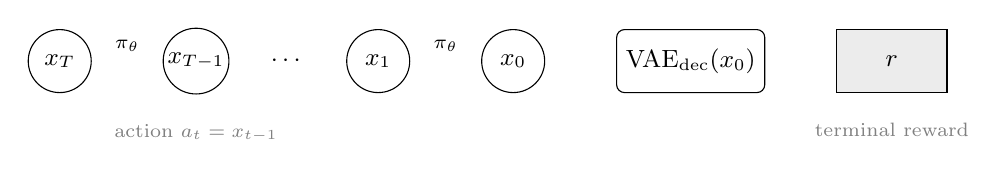
\begin{tikzpicture}[
    node distance=10mm and 9mm,
    state/.style={circle, draw, minimum size=8mm, inner sep=1pt, font=\small},
    img/.style  ={rectangle, draw, rounded corners=1mm, minimum width=10mm, minimum height=8mm, font=\small\itshape},
    rew/.style  ={rectangle, draw, fill=gray!15, minimum width=14mm, minimum height=8mm, font=\small},
    arr/.style={->,>={Stealth[length=1.6mm]}}
]
  \node[state] (xT)   {$x_T$};
  \node[state, right=of xT]   (xT1)  {$x_{T{-}1}$};
  \node[right=4mm of xT1, font=\small] (dots) {$\cdots$};
  \node[state, right=4mm of dots]   (x1)   {$x_1$};
  \node[state, right=of x1]   (x0)   {$x_0$};
  \node[img,   right=of x0]   (img)  {$\mathrm{VAE}_{\mathrm{dec}}(x_0)$};
  \node[rew,   right=of img]  (r)    {$r$};

  \path[arr] (xT)  -- node[above, font=\scriptsize] {$\pi_\theta$} (xT1);
  \path[arr] (xT1) -- (dots);
  \path[arr] (dots) -- (x1);
  \path[arr] (x1)  -- node[above, font=\scriptsize] {$\pi_\theta$} (x0);
  \path[arr] (x0)  -- (img);
  \path[arr] (img) -- (r);

  \node[font=\scriptsize, gray, below=2.5mm of xT1]   (a1) {action $a_t = x_{t-1}$};
  \node[font=\scriptsize, gray, below=2.5mm of r]     (rw) {terminal reward};
\end{tikzpicture}
\caption{The DDPO MDP. Each DDIM denoising step $x_t \to x_{t-1}$ is an action sampled from $\pi_\theta(x_{t-1}\mid x_t,c)$ with tractable Gaussian log-probability. The trajectory is decoded through the (frozen) VAE and a single scalar reward $r$ is assigned to the image. Per-step log-probabilities stored during rollout enable the PPO ratio at update time.}
\label{fig:mdp}
\end{figure}

\paragraphhead{Multi-objective reward.}
We replaced the single PickScore reward with the weighted sum of Eq.~\ref{eq:multiobj}, computed identically every PPO rollout. The components are: (i)~$r_{\pickscore}$~\citep{Kirstain23}, the CLIP-ViT-H-14 PickScore, with empirical range ${\approx}[18, 22]$ on SD-1.5; (ii)~$r_{\clipscore}$~\citep{Hessel21}, image--text cosine similarity computed from a \emph{separate} CLIP backbone (\texttt{openai/clip-vit-base-patch32}~\citep{Radford21}) so the signal is not a re-use of the policy's own embeddings, with empirical range ${\approx}[0.20, 0.35]$; and (iii)~$r_{\mathrm{diversity}}$, the per-image mean off-diagonal pairwise LPIPS~\citep{Zhang18} to the other samples sharing the same prompt:
\begin{equation}
  r_{\mathrm{diversity}}(I_i) \;=\; \frac{1}{|\mathcal{G}_p| - 1} \!\!\sum_{j \in \mathcal{G}_p,\; j \neq i}\!\! \lpips(I_i, I_j) \quad\text{for } i \in \mathcal{G}_p,\ |\mathcal{G}_p| \geq 2,
  \label{eq:diversity}
\end{equation}
with $\mathcal{G}_p$ the indices of samples sharing prompt $p$ in a rollout (and $r_{\mathrm{diversity}}{=}0$ otherwise). We use AlexNet-trunk LPIPS at $224 \times 224$ resolution (the VGG variant is too slow per rollout) and compute it in image space at the rendered $512\times 512$ output, matching the eval-time metric. We use $|\mathcal{G}_p|=4$ (four samples per prompt across four prompts per rollout; total batch 16). Per-component statistics are logged separately for analysis.

\paragraphhead{KL regularization and correctness invariants.}
We add a per-step KL term $\beta \cdot D_{\mathrm{KL}}(\pi_\theta\;\Vert\;\pi_{\mathrm{ref}})$ with $\beta = 0.01$, where $\pi_{\mathrm{ref}}$ is recovered for free by toggling \texttt{disable\_adapter()} on the PEFT-wrapped UNet (additive LoRA structure). At initialization the $B$ matrix is zero, $\pi_\theta \equiv \pi_{\mathrm{ref}}$, and $D_{\mathrm{KL}} = 0$; KL grows monotonically during fine-tuning. Three correctness properties are verified by unit tests in our codebase: log-probability consistency between rollout and update modes; PPO ratio $\rho_t \equiv 1$ prior to any gradient step (requiring \texttt{unet.eval()} during both rollout and old-log-prob caching, to suppress dropout-induced nondeterminism); and bit-exact preservation of the frozen base UNet weights after every gradient step.

% --------------------------------------------------------------------------
\section{Experimental Setup}
\label{sec:setup}

\paragraphhead{Hardware.}
Training uses a single NVIDIA L4 GPU (22~GB VRAM, Ada Lovelace) on a Google Cloud Platform \texttt{g2-standard-4} instance (4~vCPU, 16~GB RAM, 100~GB \texttt{pd-balanced} boot disk; \$0.71/hr on-demand). The $\lambdaD{=}0$ ablation was instead run on a Lambda Cloud A100 40GB (\$1.99/hr; ${\sim}3.5{\times}$ faster end-to-end). All runs are single-GPU; no model parallelism is used. An auxiliary replication of the headline finding under an independent training pipeline (described in Appendix~\ref{sec:appendix-aux}) was carried out on a separate Google Cloud V100 16GB.

\paragraphhead{Software.}
PyTorch 2.7+ on CUDA 12, \texttt{diffusers}, \texttt{transformers}, \texttt{peft}, \texttt{lpips}~0.1.4 (AlexNet trunk). Three numerical/API patches against the upstream DDPO codebase were required to reproduce: bfloat16 precision in DDIM \texttt{alpha\_bar} (default fp16 quantizes the final-step \texttt{alpha\_cumprod} to $1.0$, zeroing variance and log-prob); defensive CLIP-output extraction across the transformers~4.x$\to$5.x API change; and a PEFT-level \texttt{enable\_adapters(False/True)} fallback for LoRA toggling. Patches are released alongside the paper.

\paragraphhead{Configuration.}
All runs share: SD-1.5 + LoRA rank 4 (${\sim}797$k trainable parameters, $0.09\%$ of total), DDIM sampling with 30 inference steps and $\eta=1.0$, batch $4 \text{ prompts} \times 4 \text{ samples per prompt} = 16$ images per rollout, 1500 PPO steps, learning rate $3{\times}10^{-4}$, weight decay $10^{-4}$, PPO clip range $\epsilon = 0.1$, advantage clip $\pm 5.0$, gradient norm clip $1.0$, and KL coefficient $\beta = 0.01$ (vanilla baseline uses $\beta = 0$). Multi-objective runs use $\lambdaP = 1.0$, $\lambdaC = 20.0$, and $\lambdaD$ varied across $\{0, 2, 5, 10, 20\}$.

\paragraphhead{Eval prompts.}
Evaluation uses 14 held-out prompts grouped into three categories: \emph{constrained} (single-subject literal scenes, e.g.\ ``a chef preparing food in a restaurant kitchen''), \emph{common\_subject} (concrete objects, e.g.\ ``a blue coffee mug on a wooden desk''), and \emph{open\_ended} (abstract/creative, e.g.\ ``an abstract representation of joy''). Eval and train pools are disjoint. Every 50 training steps, $n_{\text{samples}}{=}16$ images per prompt are generated with deterministic seeds for the per-prompt PickScore mean and the mean off-diagonal pairwise LPIPS (the diversity metric).

\paragraphhead{Final-eval endpoint.}
A CUDA-OOM in the final-eval LPIPS pairwise grid at $n{=}32$ (the grid is $\binom{32}{2} = 496$ pairs) caused us to standardize on step 1450 (last in-training eval at $n{=}16$) as the canonical endpoint for multi-objective runs. Vanilla runs (no diversity-reward path) report at step 1500.

\paragraphhead{Inference settings used by every evaluation.}
All evaluations, including the ``Base SD-1.5'' reference, use the DDPO-standard inference settings (DDIM-30, $\eta=1.0$, \texttt{guidance\_scale}~=~1.0, no classifier-free guidance). This convention is shared with prior work in diffusion RL~\citep{Black23,Fan23}: high CFG suppresses the sample diversity that policy-gradient methods need for accurate gradient estimation. As a result the base-SD-1.5 column in our visual comparison appears softer than typical SD-1.5 demos but is the only methodologically consistent reference here.

% --------------------------------------------------------------------------
\section{Results}
\label{sec:results}

\IfFileExists{figures_main/table1_final_states.tex}{% Table 1 -- final-state summary across all training runs.
% Auto-generated by scripts/build_table1_final_states.py.
% Requires: \usepackage{booktabs}
\begin{table}[t]
\centering
\caption{Final-state values across all seven training runs at the canonical endpoint (step 1450 for multi-objective runs, step 1500 for vanilla). All multi-objective runs use \texorpdfstring{$\lambda_P{=}1$, $\lambda_C{=}20$ and the reported $\lambda_D$}{lambda\_P=1, lambda\_C=20, lambda\_D varied}. \textbf{Bold} marks the best value per column. `Eval Div' is the held-out LPIPS diversity averaged over 14 prompts. `Combined' is the eval-time weighted-sum reward. Step-0 baseline shown for reference (LoRA disabled, identical across runs).}
\label{tab:final-states}
\small
\setlength{\tabcolsep}{5pt}
\begin{tabular}{l@{\hspace{1.5em}}c c r r r r}
\toprule
\textbf{Run} & $\lambda_D$ & \textbf{Step} & \textbf{Raw PScore} & \textbf{Raw Div.} & \textbf{Eval Div.} & \textbf{Combined} \\
\midrule
Step-0 baseline (LoRA disabled) & --- & 0 & 19.420 & --- & 0.656 & 19.420 \\
\midrule
Vanilla DDPO, seed=7 (Columbia) & 0 & 1500 & 16.907 & --- & 0.212 & 16.907 \\
Vanilla DDPO, seed=13 & 0 & 1500 & 16.144 & --- & 0.195 & 16.144 \\
\midrule
Multi-obj $\lambda_D{=}0$ ablation & 0 & 1450 & 19.717 & 0.725 & 0.606 & 24.848 \\
Multi-obj $\lambda_D{=}2$ & 2 & 1450 & 19.376 & 0.750 & 0.636 & 25.975 \\
Multi-obj $\lambda_D{=}5$ & 5 & 1450 & \textbf{19.874} & 0.760 & 0.633 & 29.023 \\
Multi-obj $\lambda_D{=}10$ & 10 & 1450 & 19.483 & 0.792 & 0.681 & 32.650 \\
Multi-obj $\lambda_D{=}20$ & 20 & 1450 & 19.319 & \textbf{0.868} & \textbf{0.713} & \textbf{41.929} \\
\bottomrule
\end{tabular}
\end{table}
}{\IfFileExists{figures/table1_final_states.tex}{% Table 1 -- final-state summary across all training runs.
% Auto-generated by scripts/build_table1_final_states.py.
% Requires: \usepackage{booktabs}
\begin{table}[t]
\centering
\caption{Final-state values across all seven training runs at the canonical endpoint (step 1450 for multi-objective runs, step 1500 for vanilla). All multi-objective runs use \texorpdfstring{$\lambda_P{=}1$, $\lambda_C{=}20$ and the reported $\lambda_D$}{lambda\_P=1, lambda\_C=20, lambda\_D varied}. \textbf{Bold} marks the best value per column. `Eval Div' is the held-out LPIPS diversity averaged over 14 prompts. `Combined' is the eval-time weighted-sum reward. Step-0 baseline shown for reference (LoRA disabled, identical across runs).}
\label{tab:final-states}
\small
\setlength{\tabcolsep}{5pt}
\begin{tabular}{l@{\hspace{1.5em}}c c r r r r}
\toprule
\textbf{Run} & $\lambda_D$ & \textbf{Step} & \textbf{Raw PScore} & \textbf{Raw Div.} & \textbf{Eval Div.} & \textbf{Combined} \\
\midrule
Step-0 baseline (LoRA disabled) & --- & 0 & 19.420 & --- & 0.656 & 19.420 \\
\midrule
Vanilla DDPO, seed=7 (Columbia) & 0 & 1500 & 16.907 & --- & 0.212 & 16.907 \\
Vanilla DDPO, seed=13 & 0 & 1500 & 16.144 & --- & 0.195 & 16.144 \\
\midrule
Multi-obj $\lambda_D{=}0$ ablation & 0 & 1450 & 19.717 & 0.725 & 0.606 & 24.848 \\
Multi-obj $\lambda_D{=}2$ & 2 & 1450 & 19.376 & 0.750 & 0.636 & 25.975 \\
Multi-obj $\lambda_D{=}5$ & 5 & 1450 & \textbf{19.874} & 0.760 & 0.633 & 29.023 \\
Multi-obj $\lambda_D{=}10$ & 10 & 1450 & 19.483 & 0.792 & 0.681 & 32.650 \\
Multi-obj $\lambda_D{=}20$ & 20 & 1450 & 19.319 & \textbf{0.868} & \textbf{0.713} & \textbf{41.929} \\
\bottomrule
\end{tabular}
\end{table}
}{%
\begin{table}[t]
\centering
\caption{Final-state summary table placeholder. Upload \texttt{figures\_main/table1\_final\_states.tex} to populate this table.}
\label{tab:final-states}
\begin{tabular}{lcc}
\toprule
Run & PickScore & Diversity \\
\midrule
Placeholder & -- & -- \\
\bottomrule
\end{tabular}
\end{table}
}}

\subsection{Vanilla DDPO catastrophically collapses, on both seeds}
\label{sec:results-vanilla}

The vanilla baseline (PickScore as the sole reward) ends at PickScore $16.91$ and diversity $0.212$ for seed~7, and PickScore $16.14$ and diversity $0.195$ for seed~13 (Table~\ref{tab:final-states}). Both axes degrade simultaneously: held-out PickScore drops ${\sim}13\%$ below the un-fine-tuned baseline of $19.42$, and diversity drops ${\sim}70\%$ below the baseline of $0.656$. Visually (Fig.~\ref{fig:multi-prompt}, leftmost two columns) the failure modes differ between seeds (seed~7 produces uniform colored blobs, seed~13 produces high-frequency noise patterns), but the underlying dynamic is the same: the policy has reward-hacked into a narrow region that scores well on training rollouts but does not generalize. We document the temporal structure of this collapse in Section~\ref{sec:results-step400}.

\subsection{Multi-objective DDPO preserves both axes at every $\lambdaD > 0$}
\label{sec:results-multiobj}

Across $\lambdaD \in \{2, 5, 10, 20\}$, raw PickScore stays within ${\pm}0.5\%$ of baseline (range: $19.32$--$19.87$) and final eval diversity stays at or above baseline (range: $0.633$--$0.713$). The endpoints cluster tightly in the upper-right of the alignment--diversity plane (Fig.~\ref{fig:pareto}, blue/green/cyan/purple points), in stark contrast to the vanilla cluster (red, lower-left). The phase plot (Fig.~\ref{fig:phase}, right panel) shows the trajectories themselves: multi-objective runs orbit near baseline throughout training, with only small back-and-forth movement, while vanilla (Fig.~\ref{fig:phase}, left panel) shows the characteristic spiral into the collapse zone. Diversity scales roughly monotonically with $\lambdaD$ (Table~\ref{tab:final-states}), suggesting the diversity reward provides controllable, knob-like fine-tuning of the diversity axis.

\subsection{The $\lambdaD{=}0$ ablation: CLIPScore alone is nearly sufficient}
\label{sec:results-ablation}

The most informative single experiment is the $\lambdaD{=}0$ ablation (last point in the multi-objective sweep), which sets $\lambdaP = 1$ and $\lambdaC = 20$ exactly as in the rest of the sweep but drops the diversity reward entirely. This isolates the causal role of CLIPScore from that of the diversity reward.

\textbf{Result:} the run ends at raw PickScore $19.72$ and eval diversity $0.606$ (Table~\ref{tab:final-states}, orange diamond in Fig.~\ref{fig:pareto}). The catastrophic collapse is gone; the policy preserves $92\%$ of baseline diversity and exceeds baseline PickScore. There is, however, a small residual drift: $0.606$ is $8\%$ below the baseline $0.656$. Per-category breakdowns (Appendix~\ref{sec:appendix-extra-figs}, Fig.~\ref{fig:percat}) show the drift is uniform across constrained, common\_subject, and open\_ended categories, distinguishing it from the per-category staggering of the vanilla collapse.

We can read this as two distinct mechanisms:
\begin{itemize}
  \item \textbf{CLIPScore (auxiliary faithfulness signal)} is the principal mechanism preventing \emph{collapse}. Its effect is binary: with vs.\ without CLIPScore, the policy either reward-hacks into a low-diversity local optimum or it does not. This alone provides ${\sim}75\%$ of the diversity preservation we observe (closing the gap from $0.20$ to $0.61$).
  \item \textbf{Diversity reward} controls the residual \emph{diversity axis}. Its effect is continuous: increasing $\lambdaD$ monotonically increases eval diversity from $0.61$ ($\lambdaD{=}0$) through $0.68$ ($\lambdaD{=}10$) up to $0.71$ ($\lambdaD{=}20$). It contributes the remaining ${\sim}25\%$ of preservation, plus the ability to push diversity \emph{above} baseline at higher $\lambdaD$ values.
\end{itemize}
A small Pareto trade-off becomes observable only at $\lambdaD{=}20$, where raw PickScore dips to $19.32$ ($-0.5\%$ from baseline) in exchange for the highest diversity ($0.713$).

\subsection{Step-400 cross-section: collapse as phase transition}
\label{sec:results-step400}

A snapshot at step 400 (Fig.~\ref{fig:phase}, ${\sim}25\%$ of training) reveals two things the endpoint summary misses. First, the vanilla collapse is non-monotonic and seed-dependent: seed~13 has already crashed to diversity $0.150$ by step 400 while seed~7 is mid-cracking at $0.529$, only settling at $0.21$ by step 1500. The pattern looks more like a phase transition than gradual drift. Second, at the same step all four multi-objective $\lambdaD$ values are within ${\pm}0.04$ of one another on diversity, suggesting the diversity reward acts as a stabilizer against the seed-dependent collapse trajectory. Per-prompt collapse-staging analysis (Appendix~\ref{sec:appendix-extra-figs}, Figs.~\ref{fig:percat} and~\ref{fig:heatmap}) further shows that compositional ``common\_subject'' prompts collapse first under vanilla DDPO, while multi-objective preserves all categories uniformly.

% --------------- Figures ----------------------------------------------------
\begin{figure}[!htbp]
  \centering
  \figimage[width=\linewidth]{figures/fig1_diversity_trajectory.png}
  \caption{\textbf{Diversity trajectory across all runs.} Vanilla DDPO (red, both seeds) collapses LPIPS diversity from baseline $0.656$ to $\approx 0.20$ by step 1500. The $\lambdaD{=}0$ ablation (orange, CLIPScore-only) drifts mildly to $0.606$. All four $\lambdaD > 0$ multi-objective runs hold at or above baseline.}
  \label{fig:trajectory}
\end{figure}

\begin{figure}[!htbp]
  \centering
  \figimage[width=0.9\linewidth]{figures/fig5_phase_plot.png}
  \caption{\textbf{Phase plot.} Each run's trajectory through (raw PickScore, eval diversity) space, with training step encoded as line color and anchor markers at steps 0/750/1450. Vanilla runs (left, reds) spiral into the lower-left collapse zone. Multi-objective runs (right, viridis) orbit near baseline throughout training. Yellow stars mark the LoRA-disabled baseline.}
  \label{fig:phase}
\end{figure}

\begin{figure}[!htbp]
  \centering
  \figimage[width=0.85\linewidth]{figures/fig4_pareto_scaffold.png}
  \caption{\textbf{Pareto front: alignment vs.\ diversity.} Endpoint values for all seven runs. Three regimes are visible: red collapse cluster (vanilla, lower-left), orange diamond ($\lambdaD{=}0$ ablation, mild drift), and the upper-right cluster (multi-objective $\lambdaD \in \{2, 5, 10, 20\}$). $\lambdaD{=}20$ achieves the highest eval diversity at a small ($-0.5\%$) PickScore cost.}
  \label{fig:pareto}
\end{figure}

\begin{figure}[!htbp]
  \centering
  \figimage[width=0.95\linewidth]{figures/fig7_multi_prompt_grid.png}
  \caption{\textbf{Qualitative samples: 5 prompts $\times$ 6 conditions, 4 samples per cell.} All cells generated at consistent DDPO eval settings (DDIM-30, \texttt{guidance\_scale}~=~1.0); see Section~\ref{sec:setup} for why the base SD-1.5 column appears softer than typical SD-1.5 demos. Vanilla DDPO (cols 2--3) collapses to uniform outputs on both seeds with seed-dependent texture (teal blobs vs.\ high-frequency noise). Multi-objective configurations (cols 4--6) preserve prompt-faithful structure with within-prompt variation, but share an emergent stylistic shift toward painterly/atmospheric outputs that is present even in the $\lambdaD{=}0$ ablation, suggesting it is a property of CLIPScore $+$ PickScore $+$ PPO rather than of the diversity reward specifically. Additional per-prompt qualitative panels and the per-prompt $\times$ step heatmap are provided in Appendix~\ref{sec:appendix-extra-figs}.}
  \label{fig:multi-prompt}
\end{figure}

% --------------------------------------------------------------------------
\FloatBarrier
\section{Discussion}
\label{sec:discussion}

\paragraphhead{Limitations.}
(i)~\textbf{Sample size.} Vanilla baseline at $n{=}2$ seeds; multi-objective sweep at $n{=}1$ per $\lambdaD$ value. The qualitative pattern is consistent across trajectories, but tight quantitative claims would require a broader seed sweep. (ii)~\textbf{Reward proxies.} PickScore and CLIPScore are both CLIP-based proxies for human preference; we do not include human-eval. (iii)~\textbf{Step-1450 endpoint.} Standardized due to a final-eval OOM at $n{=}32$ samples; the missing 50 steps do not change our claims. (iv)~\textbf{Cross-batch vs.\ cross-prompt diversity.} Our diversity reward operates within prompt groups; inter-prompt diversity is a separate concept we don't optimize. (v)~\textbf{Single base model.} All experiments are on SD-1.5; whether the three-regime structure transfers to SDXL or other architectures is open. (vi)~\textbf{Stylistic mode shift.} Visual comparison to base SD-1.5 (Fig.~\ref{fig:multi-prompt}, leftmost column) reveals that all multi-objective configurations share an emergent painterly/atmospheric stylistic shift, present even at $\lambdaD{=}0$, that LPIPS does not detect. A complete characterization would require base-model-relative metrics such as FID-to-base.

\paragraphhead{Three-regime story and reward-hacking literature.}
Our three-regime result connects to the broader RLHF reward-hacking literature~\citep{Skalse22}. In single-reward RL the policy is free to find degenerate optima of that one reward; adding a second reward closes off many of them, because a degenerate solution must now satisfy both metrics at once. This is consistent with multi-reward findings in DPOK~\citep{Fan23} and ImageReward~\citep{Xu23}. Our ablation goes one step further by separating the two roles: the second reward is responsible for the bulk of the preservation, and the diversity term provides a controllable knob on the residual axis.

\paragraphhead{Future work.}
Natural extensions include an extended-horizon $\lambdaD{=}0$ run (does the residual mild drift compound into collapse over $5{,}000$ steps?), a structured seed sweep on $\lambdaD \in \{0, 5, 20\}$ to put confidence intervals on regime boundaries, and replacing CLIPScore with GenEval~\citep{Ghosh23} or ImageReward to test how robust the three-regime structure is to the auxiliary-reward choice.

% --------------------------------------------------------------------------
\FloatBarrier
\section{Conclusion}
\label{sec:conclusion}

We documented a failure mode of single-reward DDPO on Stable Diffusion 1.5 + LoRA that the prior literature reports only qualitatively: a catastrophic mode collapse on both seeds we tried, simultaneously degrading held-out PickScore and LPIPS-diversity by ${\sim}13\%$ and ${\sim}70\%$ respectively. We then proposed a multi-objective DDPO formulation that adds an explicit cross-batch LPIPS diversity reward, and characterized the resulting alignment--diversity Pareto frontier across $\lambdaD \in \{0, 2, 5, 10, 20\}$. A controlled ablation reveals a three-regime hierarchy: vanilla DDPO catastrophically collapses; adding a faithfulness regularizer (CLIPScore alone) prevents the collapse but allows mild residual drift; and adding the explicit diversity reward closes that drift, with monotonic $\lambdaD$-tunable control over the diversity axis at near-zero alignment cost. The mechanism separates: the auxiliary reward prevents reward hacking, and the diversity reward provides a knob over how much within-prompt variance the policy retains.

\section*{Member Contributions}
Rushil Patra: experimental infrastructure (training launcher, multi-cloud orchestration, GCS sync), the $\lambdaD{=}0$ ablation, all primary figures and tables, paper drafting.
Dev Bahl: experimental design support, baseline analysis, results comparison, and discussion synthesis.
Alimurtaza Mustafa Merchant: from-scratch DDPO re-implementation with verified correctness invariants, GCP/V100 training workflow, the auxiliary multi-objective replication described in Appendix~\ref{sec:appendix-aux}, repository hosting, and patch authorship.

\bibliographystyle{plainnat}
\bibliography{bibliography}

% --------------------------------------------------------------------------
\appendix

\section{Additional Figures}
\label{sec:appendix-extra-figs}

\begin{figure}[!htbp]
  \centering
  \figimage[width=0.9\linewidth]{figures/fig2_per_category_trajectories.png}
  \caption{\textbf{Per-category trajectories.} The same overall trajectory broken out by prompt category. Common\_subject (compositional) prompts collapse first under vanilla DDPO; multi-objective preserves all three categories.}
  \label{fig:percat}
\end{figure}

\begin{figure}[!htbp]
  \centering
  \figimage[width=0.85\linewidth]{figures/fig6_collapse_heatmap.png}
  \caption{\textbf{Per-prompt $\times$ training-step diversity heatmap.} Rows are the 14 eval prompts, sorted by vanilla collapse onset (top = collapses last). \textbf{Left:} Vanilla seed~7: prompts collapse one-by-one, with common\_subject category going first. \textbf{Right:} Multi-objective $\lambdaD{=}10$: uniform preservation across all prompts and all training steps.}
  \label{fig:heatmap}
\end{figure}

\begin{figure}[!htbp]
  \centering
  \figimage[width=0.62\linewidth]{figures/fig8_chef_strip_curated.png}
  \caption{\textbf{Visual evidence across all training conditions for one prompt} (``a chef preparing food in a restaurant kitchen''; 4 manually-curated samples per row). All cells generated at consistent DDPO eval settings (DDIM-30, \texttt{guidance\_scale}~=~1.0, no CFG). Vanilla DDPO (rows 2--3) collapses to uniform texture in both seeds. The $\lambdaD{=}0$ ablation (row 4) preserves chef-like content with painterly stylization; $\lambdaD{=}5$ (row 6) is the most prompt-faithful of the multi-objective sweep, while higher $\lambdaD$ values (rows 7--8) trade some prompt fidelity for more diverse compositions.}
  \label{fig:chef-strip}
\end{figure}

\begin{figure}[!htbp]
  \centering
  \figimage[width=0.85\linewidth]{figures/fig3_visual_headline.png}
  \caption{\textbf{The vanilla collapse cycle, on a single prompt.} Successive steps for ``a chef preparing food in a restaurant kitchen'' under vanilla DDPO (seeds 7 and 13) and multi-objective $\lambdaD{=}10$. Vanilla cycles through multiple distinct failure modes (textured noise $\to$ color blobs $\to$ solid colors); multi-objective produces faithful, varied chefs throughout.}
  \label{fig:visual}
\end{figure}

\section{Auxiliary Replication Under an Independent Pipeline}
\label{sec:appendix-aux}

To check that the headline directional finding of this paper, that an explicit per-prompt diversity reward in DDPO mitigates the diversity loss observed under preference-only training, is not specific to our primary configuration, we additionally ran an auxiliary multi-objective experiment under a separate, independently developed training pipeline. The auxiliary configuration differs from the main configuration in several respects, summarized below; we report its results in this appendix because the differences in hyperparameters and runtime budget make the numbers \emph{not directly comparable} to the main tables, but the directional behaviour is consistent.

\paragraphhead{Differences from the main configuration.}
The auxiliary pipeline trains for 500 PPO steps rather than 1500, on a Google Cloud V100 16GB rather than L4/A100, in float16 rather than the main pipeline's setup, with a smaller per-iteration batch (4 prompts $\times$ 4 samples = 16 images per rollout, identical to the main config), at learning rate $1{\times}10^{-4}$ rather than $3{\times}10^{-4}$, and with a much milder multi-objective weighting ($\lambdaP = 1.0$, $\lambdaC = 0.25$, $\lambdaD = 0.50$, $\beta = 10^{-3}$). The eval set is also different (20 prompts in the auxiliary pipeline; the same three-category stratification as the main pipeline). The diversity reward in the auxiliary pipeline uses per-image same-prompt CLIP-embedding novelty rather than LPIPS.

\paragraphhead{Result.}
Across two seeds (auxiliary run-1 on A100 bfloat16, auxiliary run-2 on V100 float16), the multi-objective configuration sacrificed approximately $0.22$ PickScore points relative to a matched PickScore-only baseline ($+0.79$ vs.\ $+1.01$ in absolute step-0-to-final $\Delta$PickScore, averaged across seeds), in exchange for a $5.3$~percentage-point reduction in CLIP-variance collapse ($-10.1\%$ vs.\ $-15.5\%$, averaged across seeds). The two seeds agree to within $0.1$~pp on the magnitude of the multi-objective improvement despite the hardware/precision asymmetry, providing weak cross-experiment replication evidence for the headline claim that an explicit diversity reward mitigates collapse at modest reward cost.

\paragraphhead{Complementary diversity metric.}
The auxiliary pipeline additionally logs CLIP image-embedding variance, a semantic-spread metric that complements LPIPS. On the auxiliary baseline, CLIP variance dropped by ${\sim}15.5\%$ from step 0 to step 500 while LPIPS dropped by only ${\sim}1.8\%$, an order-of-magnitude difference in sensitivity. This corroborates the design choice in the main paper to track diversity at the perceptual level (LPIPS) but suggests that prompt-conditional generation collapse can also be detected via semantic-spread metrics; a single LPIPS curve may understate the magnitude of a collapse that has both perceptual and semantic components.

\paragraphhead{Caveats.}
The auxiliary pipeline reaches absolute reward levels lower than the main pipeline because of its shorter training horizon (500 steps vs.\ 1500) and its much smaller faithfulness weight ($\lambdaC = 0.25$ vs.\ $20$). It does \emph{not} reproduce the catastrophic vanilla-collapse regime documented in the main paper (a 500-step run is too short to enter the $\sim$1000-step phase-transition regime visible in Fig.~\ref{fig:trajectory}), and its multi-objective mitigation is correspondingly milder. The auxiliary run is therefore best read as a directional consistency check rather than an independent replication of the three-regime hierarchy.

\section{Implementation Details}
\label{sec:appendix-impl}

The codebase implements DDIM sampling with stored per-step log-probabilities and a PPO-style update loop that iterates over denoising timesteps in shuffled order. Rollouts are generated with the UNet in evaluation mode (\texttt{unet.eval()}) to avoid dropout-related nondeterminism that would otherwise break the PPO ratio at initialization. During the inner update, stored latents are moved back to GPU one timestep at a time to bound peak memory. LoRA parameters are kept in float32 for stable optimization while the frozen Stable Diffusion components use bfloat16 (A100) or float16 (V100/L4). The VAE is decoded in float32 regardless of the rest of the model precision, because both bf16 and fp16 VAE decoding produce occasional NaN values for our latent statistics. Gradient checkpointing on the UNet is enabled \emph{after} PEFT wrapping, via \texttt{pipe.unet.base\_model.enable\_gradient\_checkpointing()}.

The multi-objective reward components are logged separately during training for analysis: per-image PickScore, CLIPScore, the LPIPS-based diversity reward, and the sampled regularization penalty toward the base policy. Three correctness invariants are enforced via unit tests: log-probability consistency between rollout and update modes, PPO ratio identically equal to one before any gradient step, and bit-exact unchanged base UNet weights after a gradient step. All three pass on CPU in under two minutes.

\end{document}
